%background
\chapter{Experiment and Analysis for Algorithm's Versatility}
From previous chapters, we have proved the algorithm in uniform binary tree. We wonder whether this evaluation process could still be useful in other types of binary trees. Therefore, in this section, we will analyze the game tree evaluation algorithm through two different types binary game tree, Fibonacci tree and skew-F tree. These experiments could help us to understand the Versatility for this algorithm.
\section{Fibonacci Tree}
\subsection{Definition}
Fibonacci tree\cite{FIBONACCI1982} is defined as a set of binary trees representing the recursive call structure of the Fibonacci computation process. It has n-1 internal nodes and n leaves. 
The root's value of Fibonacci tree is equal to the $n$th Fibonacci number. The left sub-tree should represent the computation process of $n-1$th
Fibonacci number, and the right sub-tree of root should represent the computation process of the $n-2$th Fibonacci. An Example of Fibonacci tree with height $4$ is shown below
     
\begin{figure}[H]
	\centering
	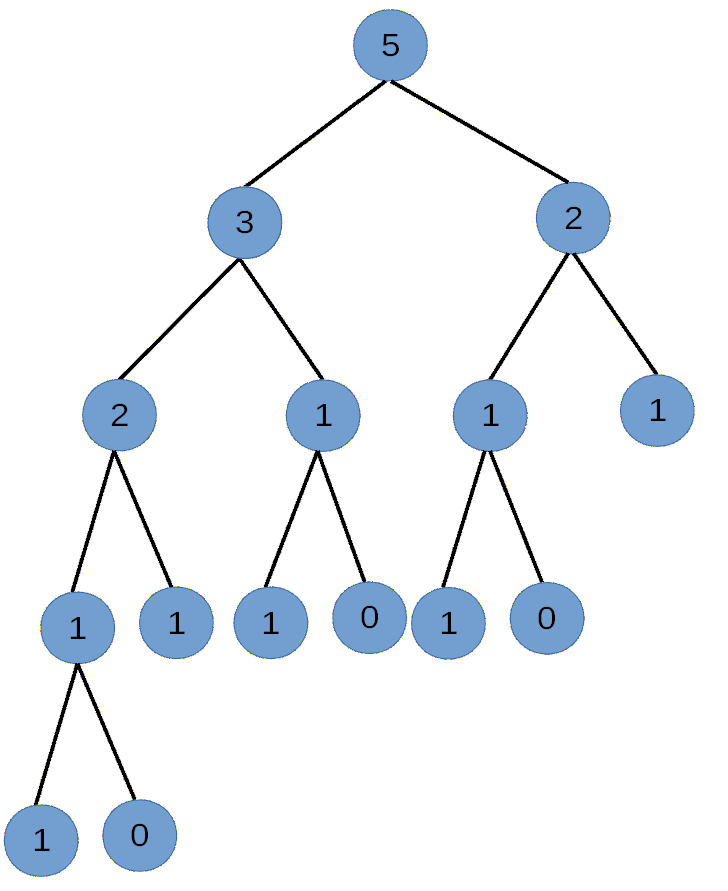
\includegraphics[width=0.5\linewidth]{fibo_tree}
	\caption{Fibonacci Tree}
	\label{fig:fibotree}
\end{figure}

\subsection{Fibonacci Tree Evaluation}
We will define a reluctant input, and let
$L(k, i)$ ($k = 0,1, 2, \dots$; $i = 0 ,1$) be 
the expected number of leaves visited by a deterministic
depth-first pruned algorithm for a Fibonacci tree of height $k$ which evaluates to true or false if $i = 1$ or $0$ respectively.
We first have that 
\begin{equation}
\label{eq:L1Fibonacci}
L(k, 1) = L(k-1, 0) + L(k-2, 0)
\end{equation}
\begin{equation}
L(0,x)=1(x=1,0)
\end{equation}


Let $p_k$ be defined recursively by $p_1 = 1/2$ and
$$\frac{p_k}{1 - p_{k}}=\frac{L(k-1,0)}{L(k-2,0)}$$.
The reluctant input is defined as follows.
If we wish that the $k$-th Fibonacci tree ($k > 0$) evaluates to 0,
then the input will make sure that at least one of the
subtrees evaluates to 0.
Specifically, the left subtree evaluates to 0 with probability $p_k$
and to 1 with probability $1 - p_k$.
Consequently, the right subtree evaluates to 0 with probability $1 - p_k$
and to 1 with probability $p_k$.


Consider first a directional algorithm that chooses
to descend to the left subtree. Its expected cost is:
$p_k L(k-1,1) + (1 - p_k)[L(k-1,0)+L(k-2,1)]$.
If instead the directional algorithm chooses to descend to the right
subtree, then its expected cost is
$(1 - p_k) L(k-2,1) + p_k [L(k-2,0) + L(k-1,1)]$, 
which by the choice of $p_k$ is the same as the cost of the algorithm
that descended to the left.

Hence, by using \eqref{eq:L1Fibonacci}, we have that
\begin{equation}
\label{eq:L0Fibonacci}
L(k,0) = p_k L(k-2,0) + (1 - p_k) L(k-1,0) + L(k-3,0) + (1-p_k) L(k-4,0)\;
\end{equation}

\iffalse
Define the sequence $\rho_k$ as the solution to the recurrence:
which could transfer to:

\begin{equation}
\rho_ka^k = \frac{a}{1+a}\rho_{k-2}a^{k-2}+\frac{1}{a+1}\rho_{k-1}a^{k-1}+\rho_{k-3}a^{k-3}+\frac{1}{a+1}\rho_{k-4}a^{k-4}
\end{equation}
\fi

Define the sequence $\rho_{k}$ as the solution to the $L(k,0)$ recurrence:
\begin{flalign}
\label{eq:Fiborhokrecursive} \rho_k &=  \frac{\rho_{k-1}}{a^2+a} +  \frac{\rho_{k-2}}{a^2+a} + \frac{\rho_{k-3}}{a^3} + \frac{\rho_{k-4}}{a^5+a^4}\\
\label{eq:Fiborhok4}         \rho_4 &= \frac{6.558171076}{a^4}\\
\label{eq:Fiborhok3}         \rho_3 &= \frac{4.512036108}{a^3}\\
\label{eq:Fiborhok2}         \rho_2 &= \frac{3.189189189}{a^2}\\
\label{eq:Fiborhok1}         \rho_1 &= \frac{2.2}{a} 
\end{flalign}

Define  
\begin{equation}
\label{eqn:L0fiboRecur} L(k,0) = \rho_k a^k
\end{equation} and $r_k$ as the recurrence vector of $\rho_{k}$
\begin{alignat*}{2}
\vect{r}_{k} & = 
\begin{pmatrix}
\rho_{k+3} \\
\rho_{k+2} \\
\rho_{k+1} \\
\rho_{k}
\end{pmatrix} &\qquad&
(k = 1, \dots )
\end{alignat*}


Then we have $\vect{r}_k=A\vect{r}_{k-1}$, where 

\begin{equation}
A = 
\begin{pmatrix}
\frac{1}{a+a^2} & \frac{1}{a+a^2} & \frac{1}{a^3} & \frac{1}{a^4+a^5}  \\
1               & 0               & 0             & 0                  \\
0               & 1               & 0             & 0                   \\
0               & 0               & 1             & 0                   \\
\end{pmatrix}\;
\end{equation}

The characteristic equation is:
\begin{equation}
\det(A-\lambda I)=\det\left(\begin{pmatrix}
\frac{1}{a+a^2} - \lambda & \frac{1}{a+a^2} & \frac{1}{a^3} &                \frac{1}{a^4+a^5}                                                \\
1               & -\lambda        & 0             & 0             \\
0               & 1               & -\lambda      & 0             \\
0               & 0               & 1             & -\lambda       \\
\end{pmatrix}\right)\;
=0
\end{equation}
which solved for $\lambda$ gets the claimed eigenvalues with
\begin{equation}
\lambda^4-\frac{\lambda^3}{a+a^2}-\frac{\lambda^2}{a+a^2}-\frac{\lambda}{a^3}-\frac{1}{a^4+a^5} = 0
\end{equation}

For $a$, with:
\begin{equation}
A \vect{v}_1 = \vect{v}_1
\end{equation}
where $\vect{v}_1$ is\footnote{This is not the vector that you use later on}
$$\begin{pmatrix}
1 \\
1 \\
1 \\
1
\end{pmatrix}\;$$
We could get:
$$ a^5 + a^4 -2 a^3 -a^2 -a -1=0 $$
Let a = $1.439650182$. 
We could get:
$$ \lambda^4 -0.284718354857539 \lambda^3 -0.095421125796929-0.335142164770774 \lambda -0.284718354857539 \lambda^2 = 0$$
whose root is:
$$\begin{pmatrix}
1.000000000 \\
-0.313238282 \\
- 0.201021681 + 0.514021596i \\
- 0.201021681 - 0.514021596i
\end{pmatrix}\;$$

We could see that the eigenvalues of A are $\lambda_1 = 1$ and other eigenvalues($\lambda_2, \lambda_3, \lambda_4$) with real part less than 0. Therefore $\vect{r}_k$ tends to the projection of $\vect{r}_1$ along an eigenvector $\vect{v}_1$ corresponding to $\lambda_1$. By using the corresponding eigenvectors to find the component r of $\vect{r}_1$ along $\vect{v}_1$, we could prove the claim. 
We could get $\vect{r}_1$ is:
\begin{alignat*}{2}
\vect{r}_{1} & = 
\begin{pmatrix}
\rho_{4} \\
\rho_{3} \\
\rho_{2} \\
\rho_{1}
\end{pmatrix} 
\end{alignat*}
By relationship:
$$\begin{pmatrix}
\vect{v}_1 & \vect{v}_2 & \vect{v}_3 & \vect{v}_4  
\end{pmatrix} 
\begin{pmatrix}
r\\
s\\
t\\
u   
\end{pmatrix} = 
\begin{pmatrix}
\rho_1\\
\rho_2\\
\rho_3\\
\rho_4
\end{pmatrix}
$$ 

We could get $r = -3.052885190463789$. Since $lim_{k\rightarrow\infty}r_k=r\vect{v}_1$ We have that
\begin{equation}
lim_{k\rightarrow\infty}\rho_{k}=-0.5r=1.52644259523189
\end{equation}

\begin{lemma}
	\label{lemma:rhok_Fibo}
	$L(k,0)$ is bounded by $L(k,0)=\rho_{k}a^k$
\end{lemma}

\begin{proof}
	Define for convenience of notation $T(k) = L(k, 0)$.
	By \eqref{eqn:L0fiboRecur} , 
	we have that $T(1) = \rho_1 a, T(2)=\rho_{2}a^2, T(3) = \rho_{3}a^3, T(4)=\rho_{4}a^4$.
	By induction process, \eqref{eq:L0Fibonacci}, and definition \eqref{eq:Fiborhokrecursive} we have $T(k)=\frac{a^{k-1}}{a+1}\rho_{k-1}+\frac{a^{k-1}}{a+1}\rho_{k-2}+a^{k-3}\rho_{k-3}+\frac{a^{k-4}}{a+1}\rho_{k-4}$, which completes the proof.
\end{proof}

By combining the lemma and recurrence relationship
we obtain the following tighter lower bound:

\begin{theorem}
	We have that 
	$\lim_{k \rightarrow \infty} L(k, 0) / a^{k} = \rho $
	and
	$\lim_{k \rightarrow \infty} L(k, 1) / a^{k-2} = (a+1)\rho$.
\end{theorem}

\section{skew F-tree}
\subsection{Definition}
A skew F-tree $S^k$is a NOR tree defined inductively: $S^k$ is a single vertex, and for every specific vertex $S^n$ in higher level will have left sub-tree as a single vertex, and right sub tree $S^{n-1}$.\citep{PROBABILISTIC}

\begin{figure}[H]
	\centering
	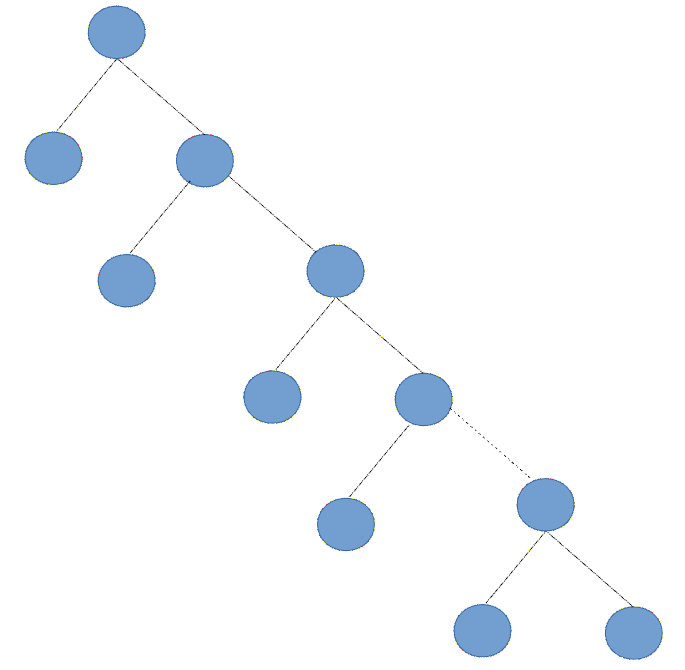
\includegraphics[width=0.5\linewidth]{skew}
	\caption{skew-F tree Example}
	\label{fig:skew}
\end{figure}

\subsection{Evaluation of skew F-tree}
From the definition in the last section, it is clear that:
\begin{flalign}
\label{eqn:skewL1} L(k, 1) &= L(k-1,0)+1\\
\label{eqn:skewLbase} L(0,i) &= 1 \quad (i = 0,1)
\end{flalign}
and also that $L(k,1) \leq k + 1$.
The reluctant input is defined as follows.
If we wish that the $k$-th Skew-F tree ($k > 0$) evaluates to 0,
then the input will make sure that at least one of the
subtrees evaluates to 0.
Specifically, the left subtree evaluates to 0 with probability $p_k$
and to 1 with probability $1 - p_k$.
Consequently, the right subtree evaluates to 0 with probability $1 - p_k$
and to 1 with probability $p_k$.
\begin{flalign}
\label{eqn:detskewL0a} L(k, 0) &= p_k+(1-p_k)(L(k-1,1)+1)\\
\label{eqn:detskewL0b} L(k, 0) &= p_k(L(k-1,0)+1)+(1-p_k)L(k-1,1)
\end{flalign}
Therefore we could have:
\begin{equation}
\label{eq:pkL0skew}p_k = \frac{1}{1 + L(k-1,0)} = \frac{1}{L(k, 1)}
\end{equation}


Consider first a directional algorithm that chooses
to descend to the left subtree. Its expected cost is \eqref{eqn:detskewL0a}
If instead the directional algorithm chooses to descend to the right
subtree, then its expected cost is
\eqref{eqn:detskewL0b} 
which by the choice of $p_k$ is the same as the cost of the algorithm
that descended to the left.

Therefore, by using \eqref{eq:pkL0skew} and \eqref{eqn:skewL1}, we could get:
\begin{flalign}
\label{eqn:skewRecur} L(k,0)=\frac{L(k-1,0)L(k-2,0)+2L(k-1,0)+1}{1+L(k-1,0)}\\
\label{eqn:skewRecur1}
L(k,1)=L(k-2,1) - \frac{L(k-2,1)}{L(k-1,1)}+2
\end{flalign}

Then we will show that $L(k,1) \ge \frac{k}{2}$ by induction:
\begin{proof}
	We start an induction with:
	\begin{flalign}
	\label{sft01}L(0,1) = 1\\
	\label{sft11}L(1,1) = 2\\
	\label{sft21}L(2,1) = 2.5\\
	\label{sft31}L(3,1) = 3.25
	\end{flalign}
	Ee could see that $L(k,1) \ge \frac{k}{2}$ stands in base condition.
	With \eqref{eq:pkL0skew}, we know that when $L(k,1)$ becomes large enough, we could say $pk = 0$. 
	Considering $L(k,0)$ when $k$ is even and large enough so we could consider $p_k$ as 0, we could have:
	\begin{flalign}
	\label{sftlbk0}L(k,0) = L(k-1,1)\\
	\label{sft1bkm11}L(k-1,1) = 1+L(k-2,0)
	\end{flalign}
	Then we could have $L(k,0) = \frac{k+1}{2}$ and $L(k,1)\ge\frac{k}{2}+1$. 
\end{proof}

In conclusion, for skew-F tree, $\frac{k}{2}+1 \le L(k,1)\le k+1$.

\subsection{conclusion}
From these two experiments, we have showed that this game tree evaluation algorithm could also be used for evaluating other types game tree for getting their lower bounds. Many other types of binary game tree could also be tested, but as the whole method is fixed, and we could prove it by Yao's principle. Therefore we could say that this game tree evaluation analysis process has versatility.